%\documentclass[a4paper, 10pt]{article}
\documentclass[paper=a4, fontsize=11pt]{article}


\usepackage[brazil]{babel}
\usepackage[utf8]{inputenc}
\usepackage{listings}
\usepackage{color}
\usepackage{amsthm}
\usepackage{graphicx}
\usepackage{cite}

\usepackage{schemabloc}
\usetikzlibrary{circuits}

\usepackage{tabularx,ragged2e,booktabs,caption}

\usepackage{hyperref}

\setlength{\parindent}{0pt}
\setlength{\parskip}{18pt}

\title{Laboratório de Maquinas de Corrente Alternada\\
Motor de Indução de Rotor Bobinado, Parte I e II}
\author{Felipe Bandeira da Silva\\1020942-X}
%\date{}

\begin{document}


\maketitle

%\newpage

%\begin{abstract}
\textit{Este laboratório tem como objetivo: identificar 
as partes externas e internas de um motor trifásico de 
rotor bobinado. Bem como o seu rotor e estator. 
Compreender o significados de corrente de excitação, 
velocidade sincrona e escorregamento com relação a um 
motor trifásico de indução. Observar o efeito do 
campo girante e a velocidade do rotor sobre  a tensão
induzida no rotor. Observar as características do motor
a vazio e em plena carga. Variação da velocidade com a 
inserção de resistência externas.}
%\end{abstract}

\newpage

\tableofcontents

\newpage

%\listoffigures


%%%%%%%%%%%%%%%%%%%%%%%%%%%%%%%%%%%%%%%%%%%%%%%%%%%%%%%%%%%%%%%%%%%%%%%%%%%%%%%%
% fundamentação teórica
\newpage
\section{Introdução}
As maquinas girantes são responsáveis por boa parte
do consumo de energia e também na sua produção. De 
acordo com ANELL a capacidade instalada para os 
geradores termoelétricos são, 

\begin{center}
    \begin{tabular}{c|c|c}
        Pais & Energia Gerada (TWh) & Parcela da Geração Mundial \\
        \hline
        Estados Unidos & 134 & 11 $\%$ \\
        Japão & 117 & 10 $\%$ \\
        Mexico & 93 & 8 $\%$ \\
        Arabia Saudita & 87 & 7 $\%$ \\
        Itália & 75 & 6 $\%$ \\
        China & 47 & 4 $\%$ \\
        Outros países & 615 & 53 $\%$ \\
        Mundo & 1168 & 100 $\%$
    \end{tabular}
    \captionof{table}{Fonte: AGÊNCIA INTERNACIONAL DE ENERGIA - AIE. Key World Energy Statistics: from the IEQ. Paris: IEA/OECD, 2003}
\end{center}

Geração esta que ocorre na utilização de combustíveis, 
em muitos casos, fosseis. Exemplo, petróleo. Esta 
necessidade ocorre no Brasil, nos tempos atuais, para
suprir a demanda nos horários de ponta, suprir
os baixos níveis dos reservatórios de agua dos 
geradoras hidroelétricas. Atendimento de sistemas
isolados. 

Tudo isto só se torna possível graças os geradores, 
maquinas girantes de grande uso. Onde foi inicialmente 
aplicado na segunda revolução industrial, com o surgimento
da energia elétrica. Como pode ser visto o motor
pode tanto ser usado para a geração de energia como de 
trabalho.

As variações para o motor de rotor bobinado são conhecidas
para proporcionarem a mudança na velocidade do eixo. Conforme
o motor aproxima-se da velocidade normal de operação, a 
resistência do reostato reduz-se gradualmente chegando a 
zero quando o motor está em máxima valocidade.

As informações teóricas para a prática são: o estador 
de um motor trifásico é conectado a uma fonte de alimentação
trifásica, a corrente que circula pelos três enrolamentos 
do estator estabelece um campo magnético girante. Gerando
três correntes, conhecidas como corrente de excitação. 
Referentes as perdas no cobre e ferro do motor. A velocidade
de campo magnético girante, também velocidade síncrona. Esta
diretamente ligada a frequência da fonte de alimentação. 
O rotor bobinado consiste de um núcleo de três enrolamento no
lugar das barras condutoras do rotor de gaiola de esquilo. O
campo magnético girante do estador induz uma tensão alternada
em cada enrolamento do rotor. Na aula prática será utilizado
um motor auxiliar para acionar o rotor, porém convém notar que, 
para uma dada velocidade do rotor, as valores de tensão 
induzida e da frequência serão os mesmos que se o rotor 
girasse por si só.

\begin{figure}[!ht]
    \centering
    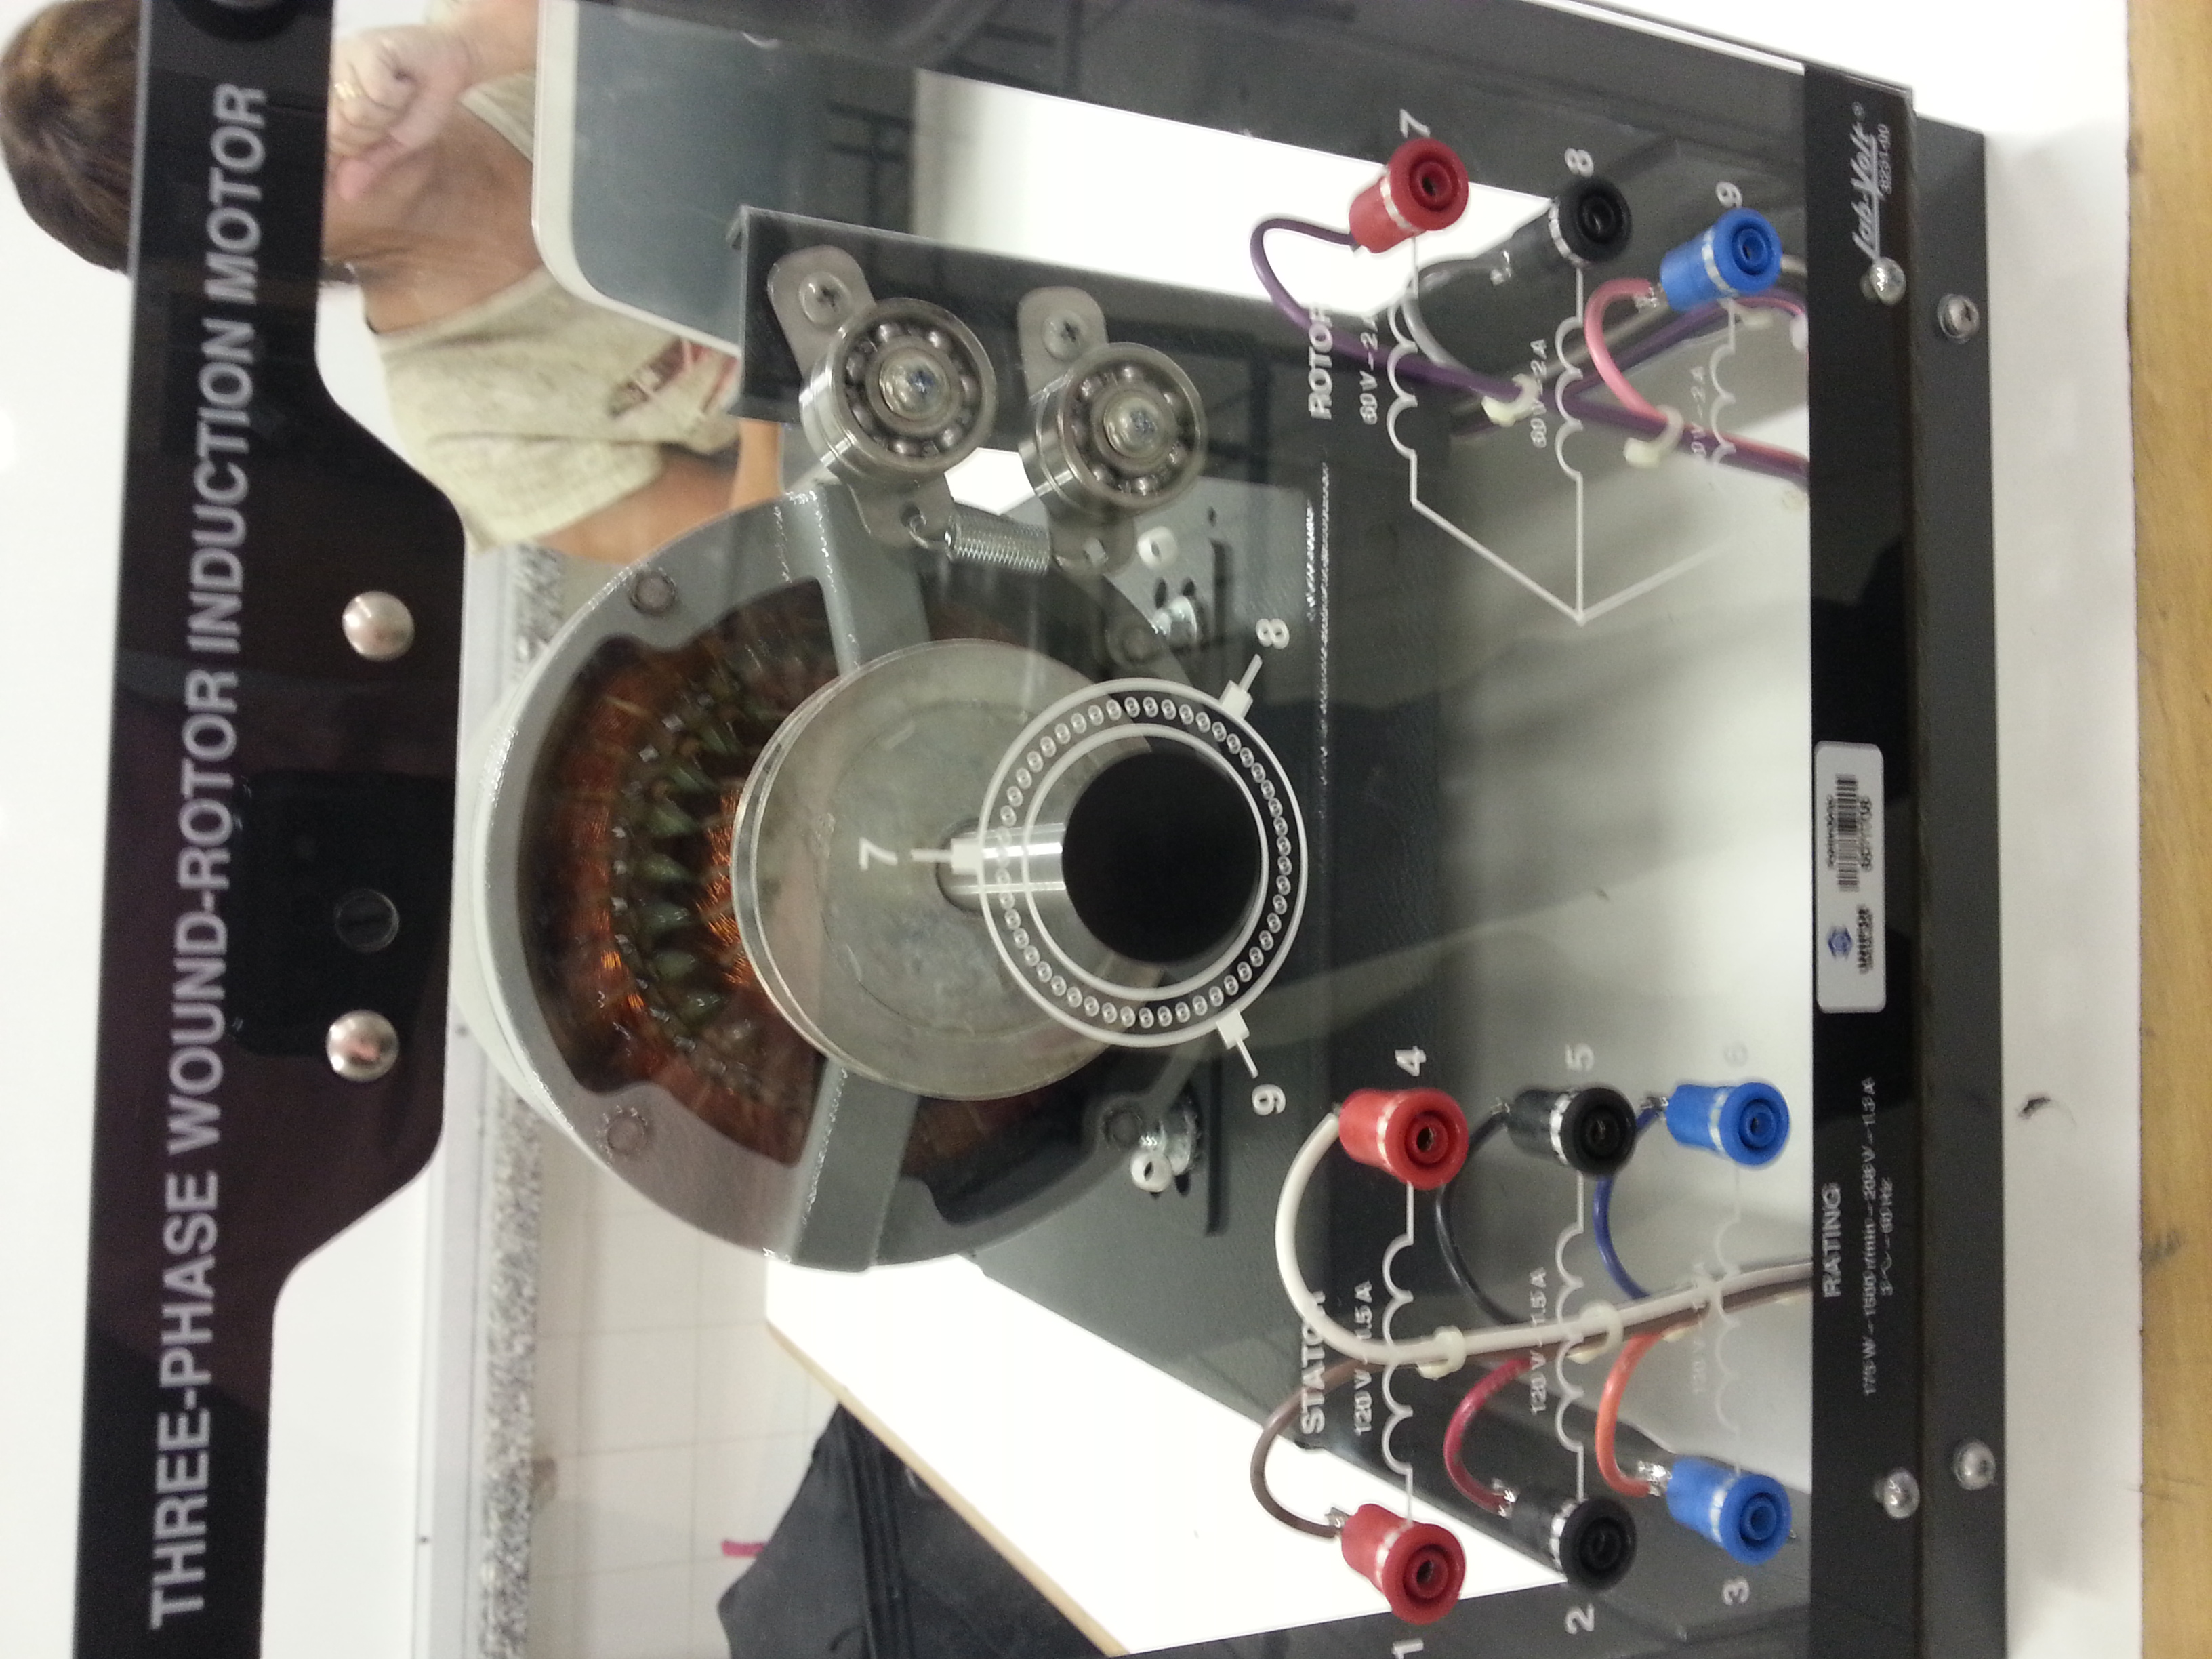
\includegraphics[scale=0.1, angle=-90]{20140326_173203.jpg}
    \caption{Motor utilizado na prática}
    \label{fig:motorutilizado}
\end{figure}

A figura \ref{fig:motorutilizado} mostra o motor utilizado
na experiência prática.

\section{Partes do Motor}

A primeira parte da experiência é no reconhecimento das partes
do motor e leitura de seus dados. A figura \ref{fig:escovasmotor}
apresenta as escovas do motor. Esta por sua fez são responsáveis
por transferir a corrente elétrica para o estator.

\begin{figure}[!ht]
    \centering
    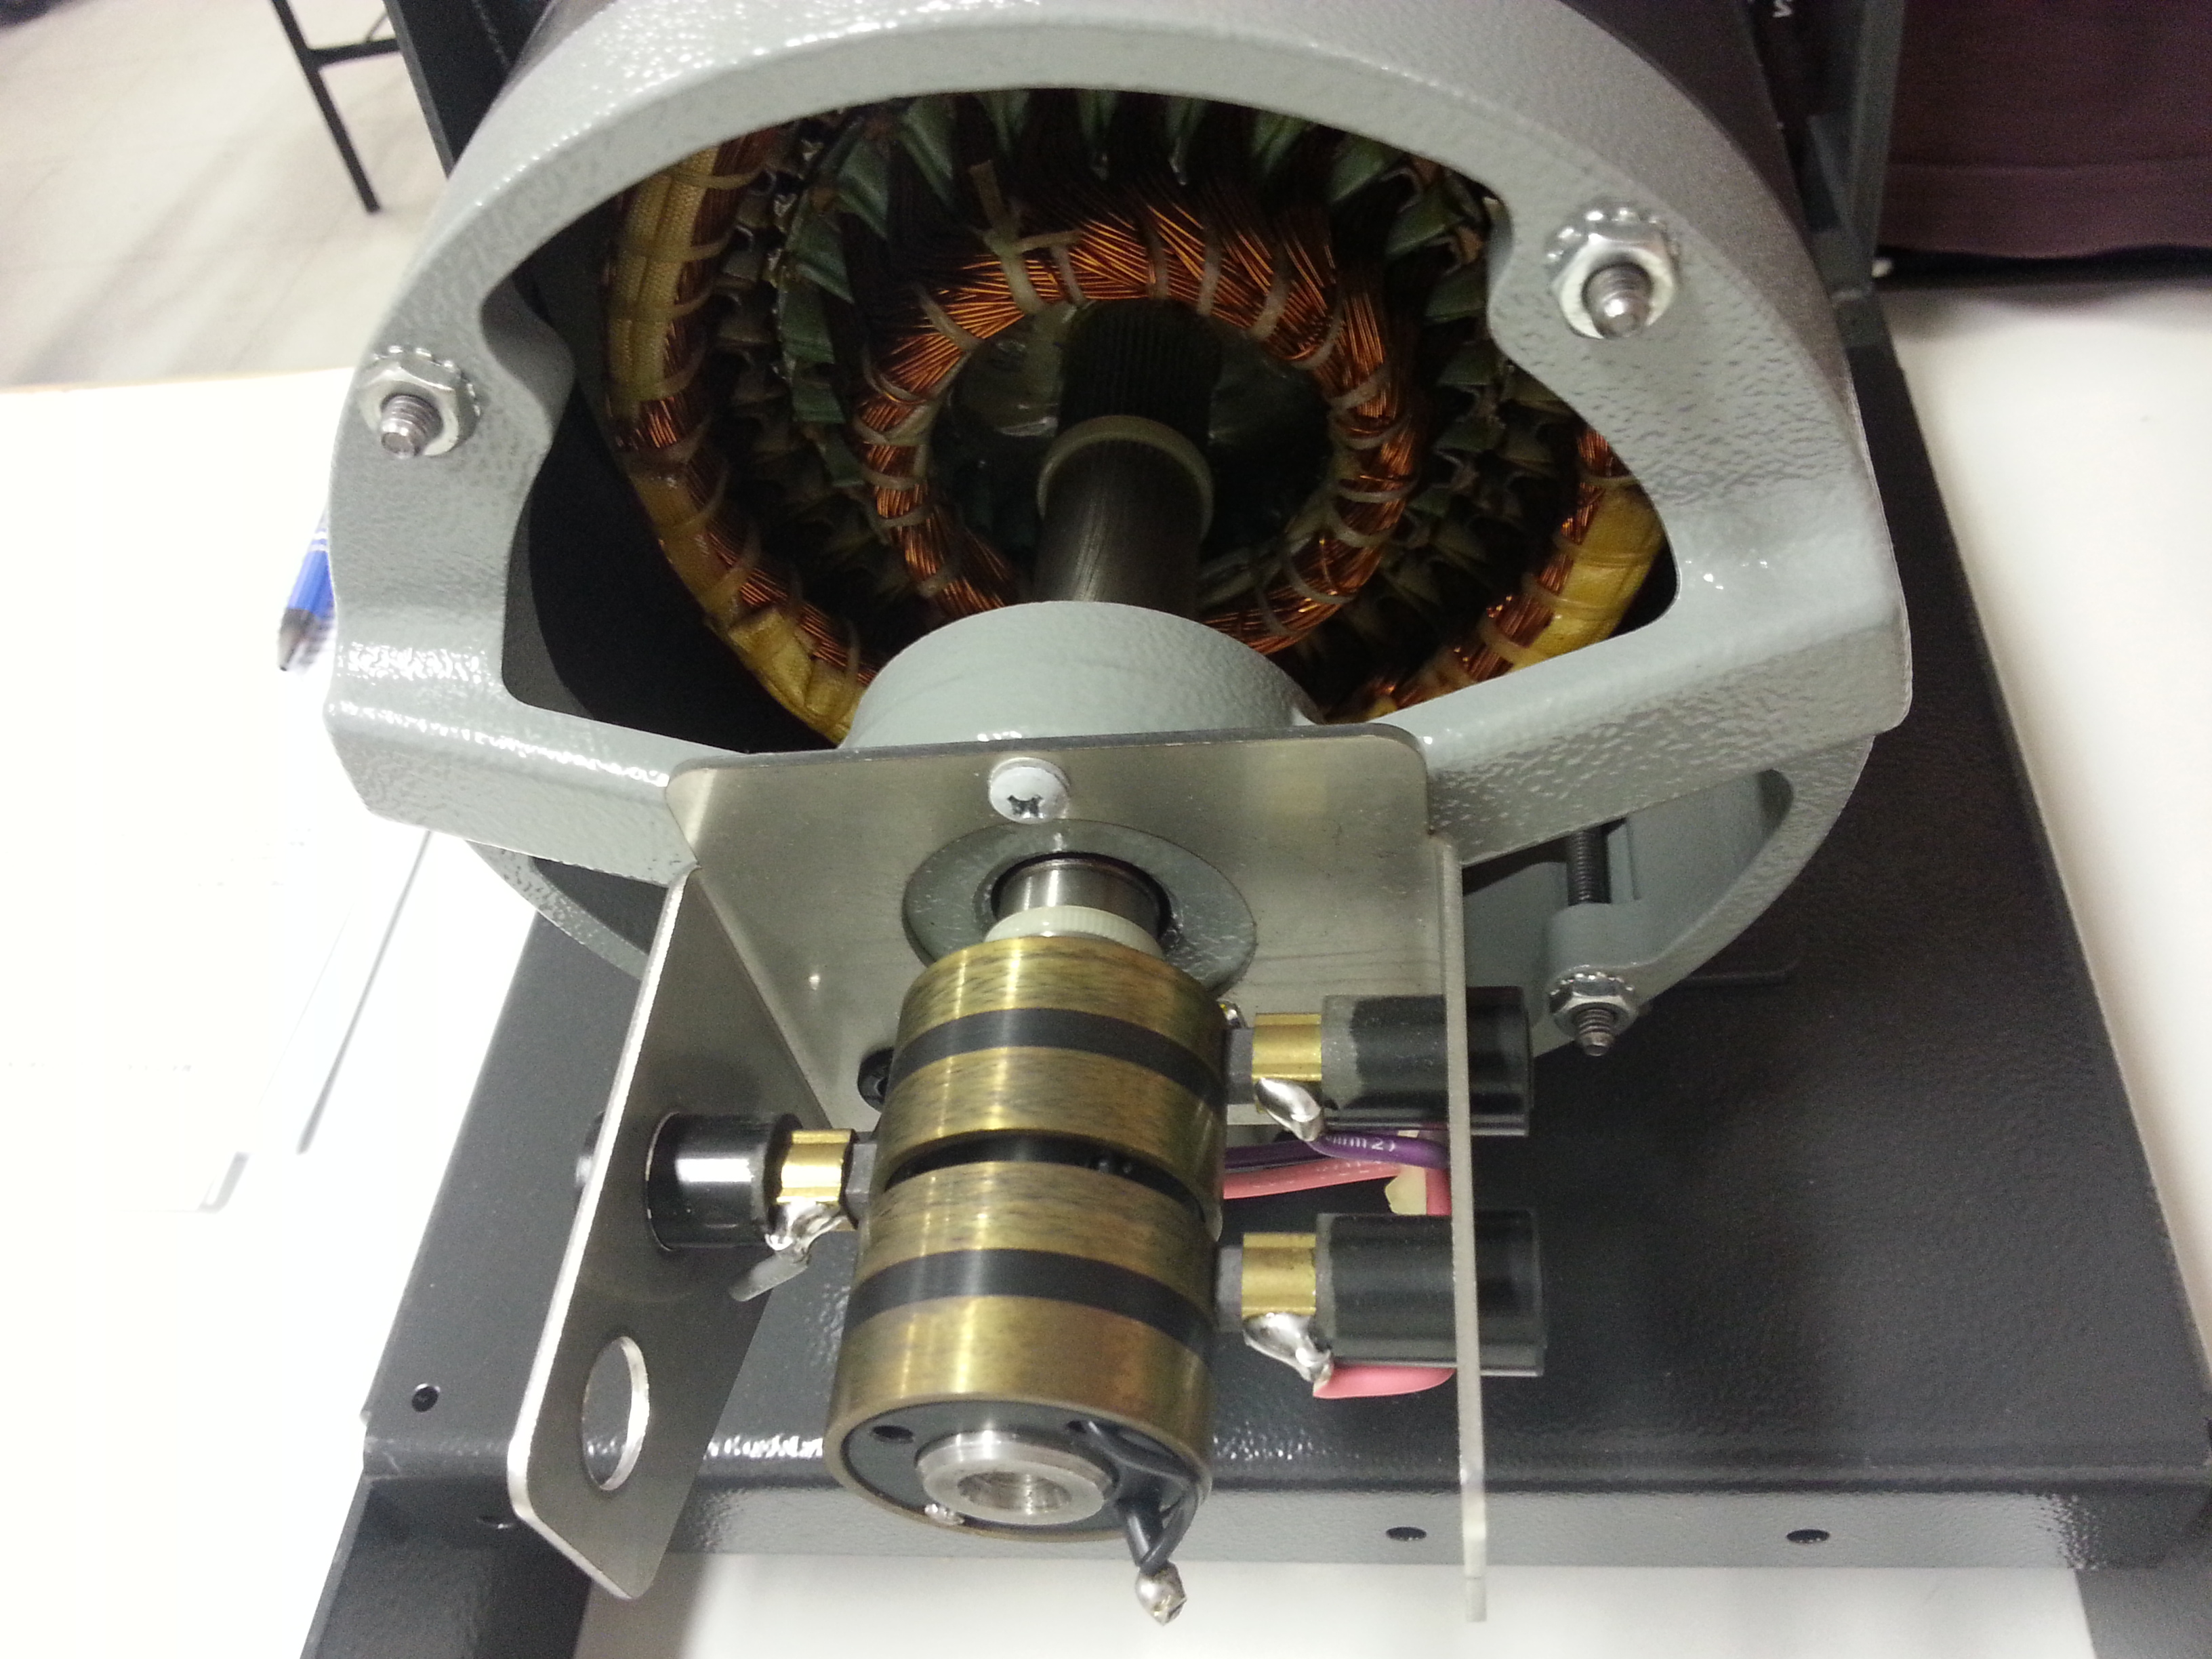
\includegraphics[scale=0.1]{20140326_172725.jpg}
    \caption{Escovas do Motor}
    \label{fig:escovasmotor}
\end{figure}

Tais escovas não podem ser movimentadas. Na mesma figura 
é possível visualizar os enrolamentos do estator, que são
os mais próximos da carcaça do motor. Os enrolamentos do
rotor que estão fixos ao eixo de rotação.

\subsection{Face Frontal}

a. Os três enrolamentos do estator estão ligados a 1-4, 2-5 e 3-6.\\
b. A corrente nominal dos enrolamentos é de 1.5 amperes.\\
c. A tensão nominal do estator é 120 volts.\\
d. Os enrolamentos do toro estão em estrela aterrado.\\
e. Estão conectados aos terminais 2, 5 e 4.\\
f. A tensão nominal dos enrolamentos do rotor é de 60 volts.\\
g. A corrente nominal do rotor é 2 amperes.\\
h. A velocidade de rotação é de 1600 rpm's.\\

\section{Montagem com motor CC de derivação}

Nesta parte se faz necessária a montagem de um 
conjuto de elementos. São eles; Motor de indução de rotor
bobinado, Motor CC em derivação e com os instrumentos
necessários para a mediação de potência(Wattímetro), 
tensão(voltímetro) e corrente(Amperímetro).

Uma fez feita a montagem, faltando aqui no relatório as 
ligações, foram obtidos os seguintes valores.


\subsection{Montando}

Acoplado o motor/gerador cc ao motor de toro bobinado por meio
da correia dentada. Mantendo a tensão c.c da armadura do 
moto/gerador em zero, ligue a fonte(o moto cc não girou).
Os seguintes dados foram obtidos. 

\begin{center}
    \begin{tabular}{c|c}
            Grandeza & Valor  \\
            \hline
            $E_1$ & 210 V \\
            $W_1$ & 0  VA\\
            $W_2$ & 0  VA\\
            $E_2$ & 96 V \\
            $I_1$ & 0 A \\
            $I_2$ & 0 A \\
            $I_3$ & 0 A\\
    \end{tabular}
    \captionof{table}{}
\end{center}

\subsection{Velocidade 900 rpm}

Agora é necessário fazer o motor chegar a 
uma velocidade de 900 rpm, fazendo variar
a tensão na armadura do motor cc.
Um fez obtida esta valor, os seguintes
dados foram medidos.

\begin{center}
    \begin{tabular}{c|c}
            Grandeza & Valor  \\
            \hline
            $E_1$ & 210 V \\
            $W_1$ & 0  VA \\
            $W_2$ & 0  VA \\
            $E_2$ & 96 V\\
            $I_1$ & 0.14 A\\
            $I_2$ & 0.16 A \\
            $I_3$ & 0.18 A \\
    \end{tabular}
    \captionof{table}{}
\end{center}

Comprava-se que o rotor esta girando no sentido
anti-horário e acompanhado o sentido do campo girante.

\subsection{Permutação da armadura cc}

Permutando as conexões da armadura c.c ao fim de inverter
o sentido de rotação do motor. E girando o restato de
campo para a posição extrema horária. Obtendo a velocidade
de 900 rpm. os seguintes dados foram medidos.

\begin{center}
    \begin{tabular}{c|c}
            Grandeza & Valor  \\
            \hline
            $E_1$ & 220 V \\
            $W_1$ & 0  VA \\
            $W_2$ & 0  VA \\
            $E_2$ & 160 V\\
            $I_1$ & 0.15 A\\
            $I_2$ & 0.17 A \\
            $I_3$ & 0.18 A \\
    \end{tabular}
    \captionof{table}{}
\end{center}

\subsection{Velocidade de 1800 rpm}

Ajustando a tensão de forma que a velocidade do rotor
seja de 1800 rpm, 

\begin{center}
    \begin{tabular}{c|c}
            Grandeza & Valor  \\
            \hline
            $E_1$ & 220 V \\
            $W_1$ & 0  VA \\
            $W_2$ & 0  VA \\
            $E_2$ & 220 V\\
            $I_1$ & 0.15 A\\
            $I_2$ & 0.18 A \\
            $I_3$ & 0.18 A \\
    \end{tabular}
    \captionof{table}{}
\end{center}

\section{Parte II, reostato de controle}

Aqui serão apresentado os dados obtidos na prática
do laboratório para o motor de rotor bobinado com
reostato de controle e uma carga eletrodinâmica.
Mensurando as potências elétricas em cada fase, 
assim como as tensões e correntes presente em
boa parte do circuito. 

Colocando o motor em uma tensão proxima de 208 volts
e ajustando as diversas cargas é obtida a seguinte 
tabela. 

\begin{center}
    \begin{tabular}{c|c|c|c|c|c|c}
            Conjudado(lbf.in) & $I_1$ & $I_2$ & $I_3$ & $WATTs$ & $VARs$ & Velociade \\
            \hline
            0 & 0.618 & 0.803 & 0.729 & 48 & 220 & 1722 \\
            3 & 0.673 & 0.878 & 0.792 & 105 & 200 & 1613 \\
            6 & 0.772 & 1.009 & 0.913 & 170 & 190 & 1600 \\
            9 & 0.903 & 1.179 & 1.092 & 240 & 190 & 1513 \\
    \end{tabular}
    \captionof{table}{}
\end{center}

Os valores para o conjudado de 12 libras-força não foi possível
já que o motor não consegue desenvolver tais potências mecânicas.

\subsection{Dial na posição extrema}

Colocando agora o dial do reostato na posição extrema, no intuito
de se obter a resistência máxima. A tabela abaixo foi obtida.

\begin{center}
    \begin{tabular}{c|c|c|c|c|c|c}
            Conjudado(lbf.in) & $I_1$ & $I_2$ & $I_3$ & $WATTs$ & $VARs$ & Velociade \\
            \hline
            0 & 0.650 & 0.791 & 0.720 & 50 & 220 & 1600 \\
            3 & 0.690 & 0.840 & 0.792 & 110 & 220 & 1400 \\
            6 & 0.786 & 0.951 & 0.915 & 170 & 210 & 1150 \\
    \end{tabular}
    \captionof{table}{}
\end{center}

Os conjudados de 9 e 12 lbf.in não foram testados já que o motor
não consegue desenvolver tais potências mecânicas. A velocidade 
do motor para todos os casos foi alterada. O torque também foi 
alterado. 

\subsection{Corrente de partida em carga plena}

O teste agora se trata na verificação da corrente máxima
desenvolvida pelo motor, em seu estado de repouso para 
a energização com carga plena. Tal teste deve ser feito
em um curto período de tempo não podendo ser feito por 
tempos demorados ou longos, por então comprometer a estrutura
física elétrica das bobinas do rotor e estator.

As seguintes corrente foram obtidas.

\begin{center}
    \begin{tabular}{c|c}
            Grandeza & Valor  \\
            \hline
            $I_1 (Amperes)$ & 1.49 \\
            $I_2 (Amperes)$ & 2.54  \\
            $E_1 (Volts)$ & 211  \\
            $Torque (N-m)$ & 0.19 \\
    \end{tabular}
    \captionof{table}{}
\end{center}

%%%%%%%%%%%%%%%%%%%%%%%%%%%%%%%%%%%%%%%%
% CONCLUSÃO
\section{Conclusão}

Conclui-se com estas duas práticas as características
inerentes aos motores de rotor bobinado, como, 
potência mecânica transferidas para ao tipos de 
cargas. Verificar visualmente o funcionamento 
de tais motores ao funcionarem sem carga e em
plena carga. Correntes de partir que excedem 
as nominais do mesmo. Variações de velocidade via
inserção de resistores variáveis.
Verificando que rotores bobinados são feitas 
para o trabalho com velocidade variáveis. 
Se são colocadas resistências no reostato, se 
faz variar o escorregamento e com isto a 
velocidade do motor. É visto que o aumento 
da velocidade provoca uma diminuição da 
potência mecânica transferida para a carga.



\end{document}
